\chapter{Introduction}
\label{chap:introduction}
% \subtitle{Building a distributed reputation system as the basic infrastructure for creating trust 
% between relative strangers for the future digital economy.}

% \paragraph{Abstract.} Trust enables cooperation which in the long-term increases welfare for all 
% parties, but centralization creates an unhealthy information and, thus, power asymmetry. The future 
% digital economy will be driven by global cooperation between relative strangers; that cooperation 
% will be facilitated by distributed reputation systems without central ownership or control. This 
% work extends the scalable TrustChain fabric with an explicit, unambiguous, public representation of 
% the entities' states, thereby making sharing of information incentive-compatbile and putting another
% pillar for the trustful internet in place.

% 1. Since the ground-breaking work of Darwin we know that evolution of species is guided by natural selection, so mutation and inheritance lead to the strongest variation surviving. However, the classic view of the strongest survives does not explain how cooperation can occur, which requires some sort of altruism. Game theory explains …
%  Nowak, Axelrod, 

Trust is the bedrock of society. From the evolution of species \cite{MOHTASHEMI2003523, nowak2006five, Axelrod1390}, economic markets \cite{akerlof1970lemons} all the way to the 
modern sharing economy \cite{resnick2002trust}, trust has always had an important impact on almost every aspect of our lives.
Trust is built on a good reputation which in turn is created through positive outcomes of past 
interactions. The value of a good reputation also depends on how widely known that reputation is.
In small communities, knowledge about each other is gained through gossiping or personal experience. 
But local communities become less important as global communities and marketplaces become more common
through internet-based applications. These larger, wide-spread internet communities lead to more
transactions of value between previously unrelated strangers. This makes a reliable trust creating
system even more important. Protecting and distributing the knowledge about transactions, that these 
systems rely on, is a tough challenge we are faced with when designing a global trust system.

The current state-of-the-art trust building systems are online platforms for the sharing economy.
The reputation systems of Uber\footnote{https://uber.com} and Airbnb\footnote{https://airbnb.com} are
an essential part of their business. The good reputation allows commuters to trust their driver and
get into the car of a stranger, or allows house owners to rent their home to a couple from the other
side of the world \cite{ert2016trust}. The reputation of drivers and renters are stored on the platforms, they are both
valuable to the people as well as the company. This leads to problems when renters do not agree with
updates to the platform: they cannot take their reputation and move to a competitor. Users are locked
into those platforms, giving their owners great power and influence.

A similar situation exists in the financial world. Banks are entrusted with their clients money, but 
their power led to corruption and the trust was abused. \cite{financial_crisis} The situation escalated in the 2007-08 
financial crisis which led to a global recession. The crisis inspired a new solution: Bitcoin \cite{nakamoto2008bitcoin}. Bitcoin
is supposed to enable secure payments without banks. Instead of centralizing power, Bitcoin distributes
the responsibility of verifying and confirming transactions over all users.
% As such it removes power from financial 
% institutions and puts it back into the hands of the actual owners of the money. 

We argue that not every digital money transaction should require a bank, and similarly not every trustful
interaction on the internet should require a third-party. Instead, the ability to prove one's trustworthiness
on the internet should be open and free for anyone. Our vision is therefore to create a universal
mechanism to create trust. This work sets an important 
step towards creating such a system. Specifically we propose a mechanism that protects and 
distributes the records of transaction which are essential for creating trust. 

This chapter introduces some key concepts offers trust and explains the context of this work.
It should shed light on the origin of trust research and its significance for the future of the 
internet. A thorough contextual basis is created for the reader to understand the problem description
and the proposed solution in the following chapters.

\section{Relevant trust research}
Virtually everyone that is part of a social community understands the concept of trust, yet defining
trust scientifically is hard. This is also due to the fact that trust is studied in a diverse set 
of sciences: evolutionary biology, sociology, economics and computer science \cite{shockley2015interdisciplinary}. In the simplified
form of a model trust can well be described and studied. The prisoner's 
dilemma \cite{rapoport1965prisoner} is one such model from game theory that creates a framework for 
understanding trust. It is widely used in research and is the basis for many experimental studies.
We describe in the following the game, it's relation with cooperation and the impact on evolutionary
theory, economics and computer networks.

\subsection{Prisoner's Dilemma}
\label{sec:prisoner}
The Prisoner's dilemma describes a dilemma common in many real-world situations, for
example the problem of two partners caught for a crime that are questioned in two separate rooms. 
Each prisoner has two options, either deny all allegations, which is more generally called cooperating
 or betray the partner, which is called defecting in general game theory. If both stay 
silent, both will get a sentence of one year. If one betrays the other, the snitch is set free while the 
betrayed gets three years in prison. If both betray each other, they both have to serve two years.
When analyzing the game without any additional knowledge and considering the payoffs for one of the
prisoner's it is always advantageous to betray the other. Either the other also betrays, in which case
two years is better than three, or the other stays silent in which case betraying sets us free. 
However, when considering both prisoners' outcomes together it would be best for both to stay silent.
\cite{rapoport1965prisoner}

\begin{figure}
    \centering
    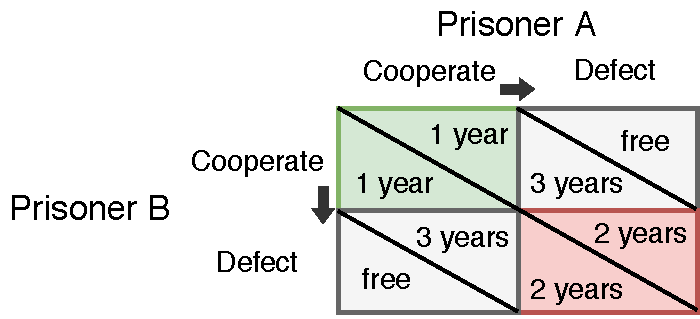
\includegraphics[width=0.7\textwidth]{images/prisoners_dilemma.pdf}
    \caption{The sentences for two prisoners in the Prisoner's dilemma. The green outcome would be 
    the best combined sentence of 2 years, while the red outcome is the worst. The arrows indicate that defecting is the dominant strategy.}
\end{figure}

While the game is quite simple the implications are far reaching. The game is able to show the 
connection between trust and \textit{cooperation}. If both prisoners trust each other to never betray a 
partner, both will cooperate and get a small sentence, the best combined outcome. Yet any mistrust
makes both fail at beating the system. The problem also describes many real world problems, called 
the tragedy of the commons \cite{Hardin1243}. For example, the global warming is a problem that can only be solved if
all peoples and all nations cooperate. Yet, the low cost and convenient usability of fossil fuels 
make it advantageous to defect and damage the environment. Either the others try to save the environment
in which case a single defection will have a small impact, or the other will also damage the environment
in which case a single cooperator will fail anyways. Only, if everyone trusts each other that
everyone does the best they can to save the environment, then it is possible to avoid the tragedy 
of the commons.

\subsection{Evolution and cooperation}
\label{sec:evolution}
While cooperating, according to theory, is not necessarily a winning strategy, it is in our nature 
to do so, as has been shown by evolution theorists. The theory about competitive natural selection 
between individuals and mutation and inheritance of genes was the accepted truth about evolution 
since Darwin until in the late 1960s doubts arose about the completeness of this 
theory. When looking at group behavior in species one will find that cooperation is a common theme
among related individuals, yet there is no place for cooperation in the classic Darwin 
theory~\cite{Axelrod1390}. In their work Axelrod and Hamilton \cite{Axelrod1390} 
analyze how to combine the seemingly inferior individual's strategy of cooperating with the goal to 
maximize fitness. At the basis of their experiments is again the Prisoner's 
Dilemma, but Axelrod and Hamilton let agents compete in multiple iterations of the dilemma. In the so-called Iterated Prisoner's Dilemma different
strategies can be tested. They found that if the game is played repeatedly with the possibility of 
meeting the same partner again in the future, cooperation between players can be established and be
superior. The best strategy was also the simplest one, called \textit{tit-for-tat}. The agent would cooperate
in the first round and afterwards imitate the partner's action.

Later research showed that this direct form of reciprocity, the act of returning a deed,
is only one form of cooperation found in human behavior. Nowak and 
Martin~\cite{nowak2006five} defined in total five forms in which cooperation can occur: kin selection, direct
reciprocity, indirect reciprocity, network reciprocity and group reciprocity. Conceptually these 
forms can be described like this:

\begin{itemize}
    \item kin selection: ``we help those that share our genes''
    \item direct reciprocity: ``I help you, you help me''
    \item indirect reciprocity: ``I help you, somebody helps me''
    \item network reciprocity: ``neighbors help each other''
    \item group selection: ``A group, in which members help each other, survives''
\end{itemize}

Each concept entails at its basis trust. We trust our family, our group, our countrymen, those with whom we had a lot
of shared experiences and those we heard good things about. 

\subsection{Direct vs indirect reciprocity}
\label{sec:indirect_reciprocity}
Especially the concept of \textit{indirect reciprocity} plays a major role in global-scale communities. The 
large size of such communities makes repeated interactions between the same partners, as in the Iterated Prisoner's
Dilemma, less likely. Instead, most interactions will be with a new person. Also, in the Prisoner's 
Dilemma both agents can help each other which is also not the general case. Instead, often person 
$A$ can help person $B$, yet $B$ cannot be useful for $A$. However, $B$ is able to contribute towards
$C$. Figure \ref{fig:indirect_reciprocity} shows this flow of contributions. At some point $C$ might
meet $A$ and be able to provide value.

\begin{figure}
    \centering
    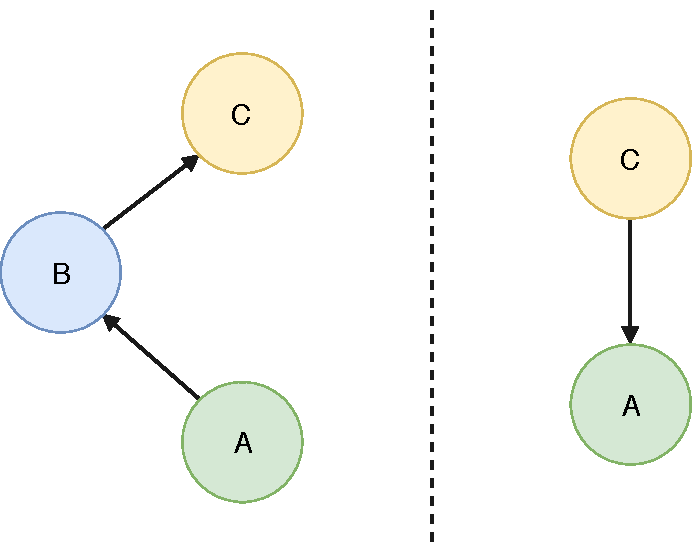
\includegraphics[width=0.4\textwidth]{images/indirect_reciprocity.pdf}
    \caption{Indirect reciprocity means that A helps B which motivates B to help C. At some point
    C meets A and may return the favor to A, knowing that A has previously helped others.}
    \label{fig:indirect_reciprocity}
\end{figure}

Therefore, a variation of the Prisoner's Dilemma game has been studied by evolution theorists, which
we will refer to this as the donation game. In it players are either donor or recipient for one round, the donor can decide to either donate
some value to the recipient or not. In subsequent rounds, players will switch roles such that they
are donor and recipient in equal number of rounds. Donating comes at a small cost but largely benefits the recipient.
In this game agents again can follow certain strategies, for example simple strategies like always donate or never
donate. A more realistic strategy is, similar to tit-for-tat, donate to other that have also donated.
If all agents donate on the first round, and knowledge of those donation is spread to other players, 
in the following rounds also all players will donate and cooperation is certain. Players who deny a
donation will also be denied by others.
Research has shown that if the costs compared to the benefit are sufficiently low and the history of
behavior of partners is sufficiently well-known to players, cooperation can be established \cite{nowak2005evolution}.

The stability of the cooperative strategy in the donation depends on the knowledge about what strategy
a partner adhered to in previous rounds. If $A$ is has donated value to $B$ and in a later round 
$C$ has to decide whether to donate to $A$, knowledge of $A$'s previous interaction influences the 
decision. If $C$ knows about $A$'s donation, $C$ will most probably also donate, otherwise this might
not be the case. This knowledge is generally known as \textit{reputation}. Through donating to others
agents build a reputation of being altruistic. If this reputation is spread, others can reward the
altruistic reputation with a donation towards them. Spreading of reputations is essential to ensure
cooperation and also happens in human society where it is known as \textit{gossiping}. We talk about
other people in order to estimate their reputation and build trust. A visualization of this process 
is depicted in Figure \ref{fig:reputation_building}. 

\begin{figure}
    \centering
    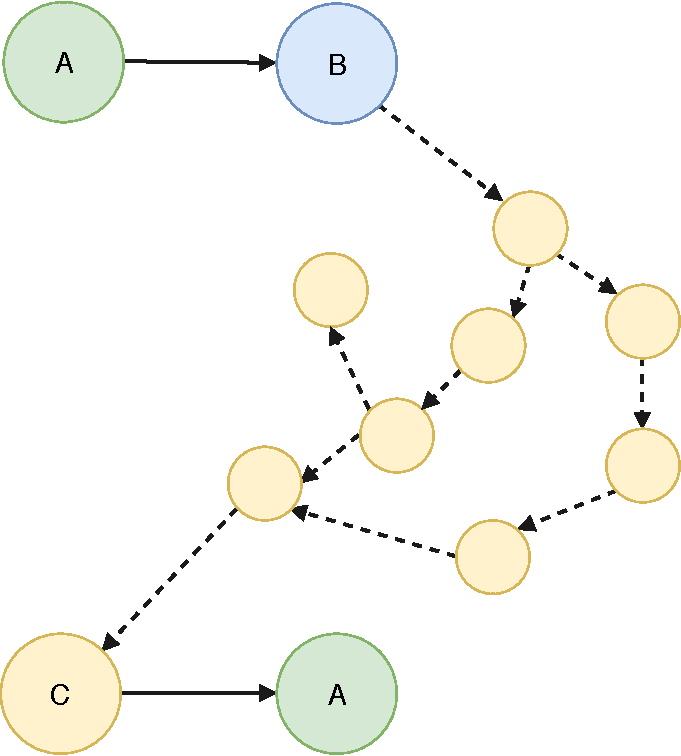
\includegraphics[width=0.4\textwidth]{images/reputation_building.pdf}
    \caption{The knowledge of a donation from $A$ to $B$ is spread through a community, building $A$'s
    reputation. $C$ hears about $A$'s reputation and donates to $A$.}
    \label{fig:reputation_building}
\end{figure}


% 2. Trust in economy and digital markets …. Advance of sharing economy, ….. When talking about trust, indirect reciprocity is the method of creating cooperation. Mui created a first mathematical model which relates reputation, trust and reciprocity. According to that model reputation stems from the history of encounters 
% Mui, Martin

\subsection{Economics}
The Prisoner's Dilemma, trust and cooperation are not only studied by evolution scientists but also
economists. A marketplace is a good example for a context in which strategies for indirect reciprocity
can be applied.
How trust and the lack of it influence trade and markets has been studied in the well-known paper ``Market for lemons'' by 
Akerlof~\cite{akerlof1970lemons}. He describes the information asymmetry between seller, who knows
the quality of the goods which will be sold, and the buyer, who can only estimate that quality by 
some market statistic. The seller's incentive to sell goods of lesser quality than the average 
statistic leads to a decreasing statistic and thus price which in turn decreases the quality of the 
goods sellers are willing to offer for that lower price. Hence the market breaks down. Akerlof
describes institutions to solve this problem namely institutions such as guarantees, brand names and
certifications. These are trust inducing institutions and can be generalized as \textit{reputation systems}.
If the sellers sell goods to many people and those people report or gossip the good quality of what
they have bought, others can trust those sellers and both seller and buyers will thrive. On the 
other hand a bad reputation will lead to a seller getting out of business as buyers will mistrust.
This closes the gap to the work of Nowak as this reputation is what makes indirect reciprocity
possible: the seller is not taking advantage of the buyer's inconvenient situation but the buyer
cannot directly return that favor. Only by gossipping the event to other potential buyers who are 
then more willingly to buy from the seller is the reciprocity circle closed.~\cite{nowak2006five}

% 3. Reputation systems guide buyers towards to most trustworthy sellers on markets or help guests find houses on Airbnb that actually hold the promises made in the description. Reputation systems require three properties: dissemination, strong identities and  Yet companies take advantage of our trust and misuse our data, influence us and do not take appropriate measures to protect our data from attacks. Centralized systems are broken.
% (eBay) Ba and Pavlou, survey of reputation systems, definition of reputation system, Pouwelse 
\section{Evolution of trust systems}
Although the role of trust for marketplaces is well described by the market for lemons, the ways of 
building trust have evolved as shown in Figure \ref{fig:economy}. In the pre-industrial age, most economy and trade was done in local
communities with families that trusted each other over generations and traders that returned year
after year. Trust was mostly based on personal experience or word-of-mouth marketing. 

\begin{figure}[h]
    \centering
    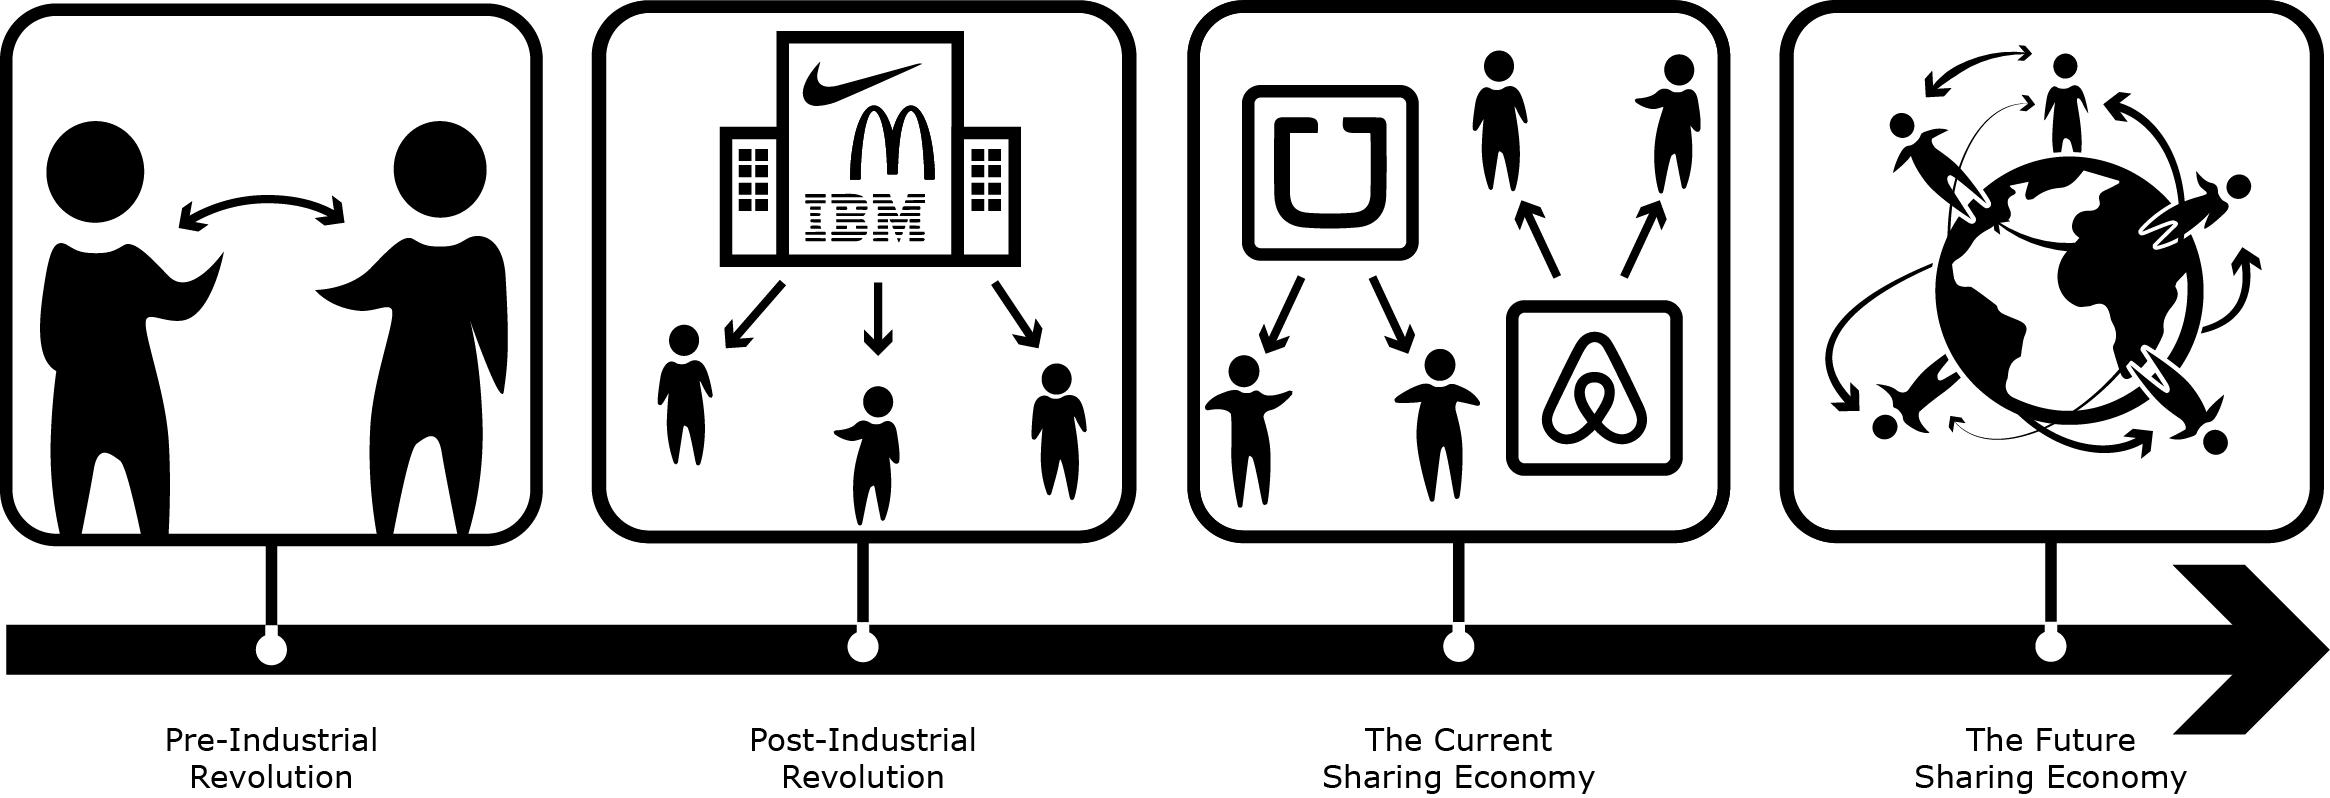
\includegraphics[width=\textwidth]{images/economy.png}
    \caption{Evolution of the economy. Source: Created at Blockchain Lab TU Delft}
    \label{fig:economy}
\end{figure}

During industrial and post-industrial age companies have largely replaced local producers and are 
trusted by millions of customers based on their brand name. We buy most goods from nation wide and 
global companies that are competing with few other competitors. Trust is build through advertisements
and product quality but also the effect of masses plays a role: if many people have an iPhone, even 
more people want one. But the trust has limits. A recent example of a company misusing the trust in 
the brand is Volkswagen~\cite{VWDiesel}, who advertised and sold dirty Diesel cars under the cover 
of being clean. 

The last two decades saw the development of a new branch of the economy: the sharing economy powered
by the internet. We can now buy used goods on eBay, renting a house to a stranger (or from a 
stranger) on Airbnb, get into a stranger's car with Uber. The sharing economy or collaborative consumption is the 
rising star of economic concepts in the information age and it is powered by reputation. A company 
offers a platform on which the two sides of a trade or transaction can find each other. With each 
encounter both parties can rate that interaction and it becomes part of their history. With a longer
and more positive history the value of a profile increases as users see the reputation as security
for a good interaction and are willing to pay for it. However, there are reasons for concern. What
if the platform changes their rules in an almost unacceptable way or abuses the personal data their
users have entrusted them with? Users cannot take their reputation and data to another platform
because their reputation is actually owned by the platform facilitating the trades. Similar to what
can be seen in the analog economy, digital companies first build trust with their users before 
abusing their power. Again a recent example is the facebook/cambridge analytica scandals.~\cite{facebook} 


Similar to the above examples of a misuse of trust, customers of banks lost trust in them when large
scale speculations in the housing market led to the 2008 financial crisis\cite{financial_crisis}. 
Shortly afterwards an alternative financial system was proposed with Bitcoin\cite{nakamoto2008bitcoin}.
Bitcoin enables digital money transfers without banks, so direct transactions between owners of 
bitcoins in a decentralized system. The advent of Bitcoin represents the next step in the digital
economy, in which market interactions happen directly between entities without an intermediary.


% 4. The above discussion makes clear that the future digital economy requires a distributed reputation system. But making a reputation system distributed brings many additional challenges. A distributed system has no control entity which can enforce strong evidence for identities. Also single entities in a distributed system have most commonly no full view of the network, thus are not aware of all other entities or all encounters. The field is not entriely new but distributed reputation systems have been researched especially in the context of peer-to-peer file-sharing, and mobile ad-hoc system. Donation game is the game-theoretic model for this …. Although a lot of research has been conducted in the field of distributed reputation systems, major problems like the Sybil-attack, double spending, scalability and state consistency remain largely unsolved.
% Game-theoretic modeling of reputation

We envision a future in which collaborative consumption is possible through direct trustful connections. This
future requires a trust system which is application agnostic, owned by no one and ruled by 
everyone: a distributed system as a layer directly on top of the internet. However this poses some 
challenges from a technical point of view. Distributed system are intrinsically hard to control and regulate, which is both 
blessing and curse. No party can impose unfair rules on other users but it is also hard to prevent 
malicious users from sending wrong information across the network. Mechanisms need to be designed to
encourage honest behavior in the system. Although Bitcoin has proven that secure interactions in a
distributed network are possible it struggles with major scalability issues.\cite{gervais2016security}
Distributed, secure and globally scalable systems remain an unsolved problem. 

% 5. This master thesis was written in the context of the blockchain lab at TU Delft which has a long history of research on the topic of distributed reputation systems. The research is targeted at Tribler, a secure BitTorrent client which is aimed at protecting against free-riders.
% BarterCast
\section{Tribler and its relation to trust systems}
\label{sec:tribler}
Distributed trust and reputation systems are not completely new. Examples of reputation systems
being applied in a distributed application can be found in the field of peer-to-peer
data exchanges and mobile ad hoc networks. \cite{HENDRIKX2015184} In both contexts a reputation system
can ensure the fair use and contribution to the network's pool of resources. In this section we 
introduce Tribler, a peer-to-peer file-sharing and video streaming service which is based on the 
BitTorrent protocol. Taking Tribler as an example, we show how an application context can be mapped to 
the dilemma and trust problem which were discussed so far.

\begin{figure}
    \centering
    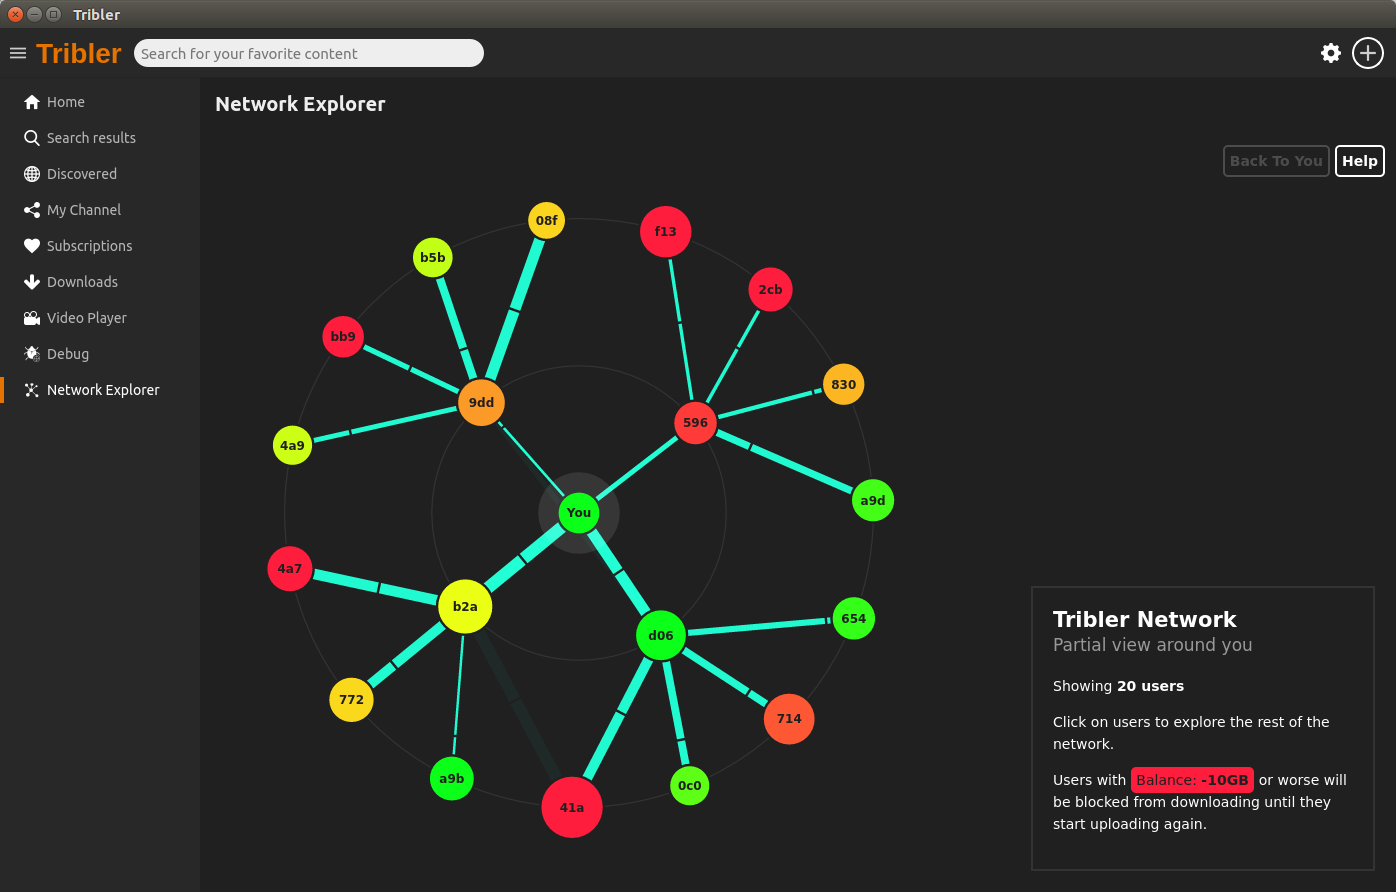
\includegraphics[width=0.7\textwidth]{images/tribler}
    \caption{Graphical user interface of Tribler. The network graph shows which nodes we have 
    interacted with in the past. The stroke width of the connections shows their reputation from 
    our point of view.}
    \label{fig:tribler}
\end{figure}

\subsection{Trust and reputation}
The uploading and downloading of data in Tribler is a social dilemma as each user wants to 
stream videos while contributing as little as possible.
The peer-to-peer video streaming use case can be mapped to the donation game we described in 
Section \ref{sec:indirect_reciprocity} very well. When a node streams a video, it downloads the video
data from another node which has that content available. The other node needs to upload the video to
the downloader. The uploader matches the donor, while the downloader is the recipient. The uploader
does not immediately benefit from uploading a video. He only benefits if the knowledge about the 
altruistic act is spread such that he is more likely to also be able to stream videos in the future.

The reputation of an agent in Tribler then represents the 
contribution behavior of that agent. Contributing, that is uploading video streams to other users,
increases an agent's reputation whereas downloading, that is streaming videos, decreases an agent's 
reputation. Also, relaying is a neutral activity in terms of the upload-download ratio, yet the 
reputation of an agent that relays a lot of data needs to be higher as well. In contrast to 
reputation, trust is subjective and can be seen as the subjective perception of a peer being a 
``good contributor''. 

In order to better illustrate the difference between reputation and trust we provide an example.
Assume an agent $A$ knows two agents, $B$ and $C$ and sees that both have uploaded and downloaded 
the same amount of data. However, $B$ has uploaded most to $A$ while $C$ has uploaded only to 
agents that $A$ has not heard of. Human intuition tells us that $A$ should trust $B$ more than $C$, 
because of the stronger direct connection. Trust therefore depends on the topology of the network.

\subsection{Agents}
In the iterated Prisoner's Dilemma, agents are the entities that take part in games. Intuitively one
would assume that users are the agents in Tribler. It would be more accurate though to say that a 
running instance of the Tribler software is the agent. A single human user can have multiple 
instances of the software running on multiple machines and thus ``control'' multiple agents. Despite
being able to run or stop the agents, the human user has only a very small decision space, though, 
because the software runs on its own and executes according to design. 

The distinction of honest, cooperating and dishonest, defecting agents is then made as follows: honest agents are the 
instances that run the software as intended while dishonest agents are instances of manipulated 
software. 

In the following description of the system we will use both, ``node'' and ``agent'' when referring to the 
behavior of a Tribler instance executing some action. 

\subsection{Building and spreading reputations}
As explained in Section \ref{sec:indirect_reciprocity} building and spreading the reputation is 
important for cooperation to be possible. A distributed system does not allow for a central storage
or communication tool to track and disseminate reputations. Instead, a solution similar to the
human-to-human gossip is necessary to spread knowledge of previous transactions. Similar to humans, 
Tribler instances can communicate with each other, thus spreading knowledge of contribution behavior
seems to be straightforward. 

We argue that the opposite is true. As the reputation bears value, agents can try to misreport 
transactions in order to generate a better reputation than when being honest. Agents can also create
fake reports of transactions with non-existent agents or distribute conflicting reports. We need to
explore how transactions should be recorded and disseminated in order to ensure that bad 
reports and dishonest agents can be identified and dealt with.

% \section{TU Delft Blockchain Lab research}
% The ambition of creating the first global trust system\footnote{An elaborate formulation of our lab goal can be found here: https://github.com/Tribler/tribler/issues/3571} is realized at the Blockchain Lab of TU Delft,
% which is the research group in which this thesis was created. The lab has a strong focus on exploring
% new concepts, implementing them and testing them in production grade software. 

% The research group has great experience and a solid track record in the field of distributed work 
% systems. Especially peer-to-peer file sharing system have been studied, first and foremost the 
% internally developed Tribler\footnote{https://tribler.org} application. Tribler is a client for the
% BitTorrent protocol. It offers many improvements over conventional BitTorrent clients like improved
% privacy and security, streaming and reputation management. It has been the testbed for algorithms of
% bachelor, master and Phd students for ten years with 1 million downloads in that period. In those 
% years of research several milestones have been reached. In \cite{meulpolder2009bartercast} we have 
% solved the free-riding problem in the peer-to-peer file-sharing context with a reputation system 
% that tracks uploads and downloads. With TrustChain \cite{OTTE2017} we have created our own 
% blockchain fabric for bandwidth as a currency which builds on the previous work and adds 
% tamper-proof recording and immutable history to the reputation system.

% The problem of peer-to-peer file sharing systems maps well onto the trust domain. Users of BitTorrent
% clients download from other users who upload data. Downloading data has benefit to users because 
% they are interested in the content, however uploading has no obvious advantage. It is only necessary
% to keep the content available for others. There is an obvious incentive problem, a tragedy of the 
% commons. A free-rider can download without uploading, thereby consume resources without contributing.
% The problem can be solved through a trust system. By recording the behavior of each user and making
% it public a reputation can be assigned to each user which represents their resource usage. Users 
% that contribute a lot increase their reputation while downloading decreases that reputation. Other 
% users are able to inspect that past behavior of any potential partner and use it for their decision 
% whether the partner deserves a contribution. 

% The recording of file transactions and security of those records is facilitated by our blockchain
% fabric TrustChain~\cite{OTTE2017}. TrustChain is a multi-chain fabric which lets each user create
% an own chain. It is therefore built for horizontal scalability and unbounded throughput. By design,
% TrustChain enables the creation of trust in any application context. The solution is implemented
% in Tribler and has been used in production for more than a year as of 2018. The implementation 
% details of TrustChain will be discussed more in Chapter~\ref{chap:implementation}. 

% The great scalability of TrustChain comes at the cost of security. The architecture allows for 
% attacks to be detected but the system can only be secured if honest users engage in that defensive 
% behavior. This can only be ensured through incentives: agents should never be able to gain an 
% advantage by circumventing the rules. 

\section{Our contributions}
In this work we study a mechanism to ensure the proper dissemination and verification of transaction
records. In any trust system, the transaction records are the basis for the reputation of users and 
thus the trust users have in each other. We show that current approaches are either not scalable 
enough or cannot guarantee the detection of manipulation attempts. We claim that a scalable solution
requires proper incentives which encourage each agent on the network to help defend the system through
sharing and verifying the records of transactions. Specifically this work extends our TrustChain 
architecture with a new type of record: exchange blocks. Together with transaction blocks these 
enable our system to document all communication between agents. This enables the honest agents to 
verify that their peers follow the proper exchange and verification policies. We further implement
this architecture and show that if hoenst agents follow a policy to exchange all data, they are 
able to detect and ignore exchange free-riders, strategic manipulators and colluding agents, who do 
not verify their partners.

We will enlarge on the problem description in the next chapter. Afterwards TrustChain is introduced
and explained. In Chapter \ref{chap:model} we theoretically study the importance of gossiping and 
ways to prevent any free-riding on the security offered through peers. Next, we define our extension
to the TrustChain fabric and propose a specific mechanism of exchanging data. Finally, we confirm the 
ability of defending against manipulation and free-riding in experimental analysis. 
The final chapter concludes the work and makes suggestions for further research.